\section{Circular Permutations and Permutations with Similar Elements}

In this section you will learn to:
\begin{enumerate}
    \item Count the number of possible permutations of items arranged in a circle.
    \item Count the number of possible permutations when there are repeated items.
\end{enumerate}

In this section, we will address the following two problems:
\begin{enumerate}
    \item In how many different ways can five people be seated in a circle?
    \item In how many different ways can the letters of the word MISSISSIPPI be arranged?
\end{enumerate}

The first problem comes under the category of Circular Permutations, and the second under Permutations with Similar Elements.

\subsection{Circular Permutations}

Suppose we have three people named A, B, and C. We have already determined that they can be seated in a straight line in \( 3! \) or 6 ways. Our next problem is to see how many ways these people can be seated in a circle. We draw a diagram.

\begin{center}
    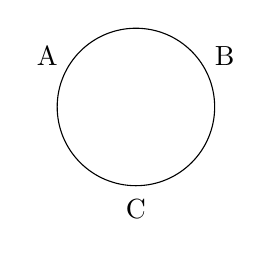
\begin{tikzpicture}
        % Draw the circle
        \draw (0,0) circle (1cm);

        % Add labels at specified angles
        \node at (150:1.3cm) {A};
        \node at (30:1.3cm) {B};
        \node at (-90:1.3cm) {C};
    \end{tikzpicture}
    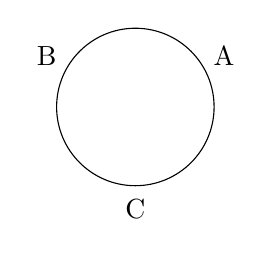
\begin{tikzpicture}
        % Draw the circle
        \draw (0,0) circle (1cm);

        % Add labels at specified angles
        \node at (150:1.3cm) {B};
        \node at (30:1.3cm) {A};
        \node at (-90:1.3cm) {C};
    \end{tikzpicture}
\end{center}

It happens that there are only two ways we can seat three people in a circle, relative to each other’s positions. This kind of permutation is called a circular permutation. In such cases, no matter where the first person sits, the permutation is not affected. Each person can shift as many places as they like, and the permutation will not be changed. We are interested in the position of each person in relation to the others. Imagine the people on a merry-go-round; the rotation of the permutation does not generate a new permutation. So in circular permutations, the first person is considered a place holder, and where they sit does not matter.

\begin{summarybox}{Circular Permutations}
    The number of permutations of \( n \) elements in a circle is \( (n-1)! \).
\end{summarybox}

Another way to look at this is to say that there are $n!$ ways to place the people around the circle, but we have to divide by $n$ because there are $n$ different people to consider the start.

\begin{example}
    In how many different ways can five people be seated at a circular table?
\end{example}

\begin{solution}
    We have already determined that the first person is just a place holder. Therefore, there is only one choice for the first spot. We have

    \[
        \begin{array}{|c|c|c|c|c|}
            1 & 4 & 3 & 2 & 1 \\
            \hline
        \end{array}
    \]

    So the answer is 24.
\end{solution}

\begin{example}
    At a scholarship dinner, there are four professors and four students. How many ways are there to sit if they want to sit alternately?
\end{example}

\begin{solution}
    We again emphasize that the first person can sit anywhere without affecting the permutation.

    So there is only one choice for the first spot. Suppose a student sat down first (since they're generally hungrier). The chair to the right must belong to a professor, and there are 4 choices. The next chair belongs to a student, so there are three choices and so on. We list the choices below.

    \[
        \begin{array}{|c|c|c|c|c|c|c|c|}
            1 & 4 & 3 & 3 & 2 & 2 & 1 & 1 \\
            \hline
        \end{array}
    \]

    So the answer is 144.
\end{solution}

\subsection{Permutations with Similar Elements}\label{subsection_permutations_with_similar_elements}

Let us determine the number of distinguishable permutations of the letters ELEMENT. Suppose we make all the letters different by labeling the letters as follows.

E$_1$LE$_2$ME$_3$NT.

Since all the letters are now different, there are $7!$ different permutations.

Let us now look at one such permutation, say

LE$_1$ME$_2$NE$_3$T

Suppose we form new permutations from this arrangement by only moving the E's. Clearly, there are $3!$ or 6 such arrangements. We list them below.

\begin{align*}
     & \text{LE$_1$ME$_2$NE$_3$T} \\
     & \text{LE$_1$ME$_3$NE$_2$T} \\
     & \text{LE$_2$ME$_1$NE$_3$T} \\
     & \text{LE$_2$ME$_3$NE$_1$T} \\
     & \text{LE$_3$ME$_1$NE$_2$T} \\
     & \text{LE$_3$ME$_2$NE$_1$T}
\end{align*}

Because the E's are not different, there is only one arrangement LEMENET and not six. This is true for every permutation.

Let us suppose there are \( n \) different permutations of the letters ELEMENT.

Then there are \( n \cdot 3! \) permutations of the letters E$_1$LE$_2$ME$_3$NT.

But we know there are \( 7! \) permutations of the letters E$_1$LE$_2$ME$_3$NT.

Therefore, \( n \cdot 3! = 7! \)

Or \( n = \frac{7!}{3!} \).


\begin{summarybox}{Permutations with Similar Elements}
    The number of permutations of \( n \) elements taken \( n \) at a time, with \( r_1 \) elements of one kind, \( r_2 \) elements of another kind, and so on, is given by
    \[
        \frac{n!}{r_1! \, r_2! \, \dots \, r_k!}
    \]
\end{summarybox}

\begin{example}
    Find the number of different permutations of the letters of the word MISSISSIPPI.
\end{example}
\begin{solution}
    The word MISSISSIPPI has 11 letters. If the letters were all different there would have been \(11!\) different permutations. But MISSISSIPPI has 4 S's, 4 I's, and 2 P's that are alike.

    So the answer is \[\frac{11!}{4!4!2!} = 34,650.\]
\end{solution}

\begin{example}
    If a coin is tossed six times, how many different outcomes consisting of 4 heads and 2 tails are there?
\end{example}
\begin{solution}
    Again, we have permutations with similar elements.

    We are looking for permutations for the letters HHHHTT.

    The answer is \[\frac{6!}{4!2!} = 15.\]
\end{solution}

\begin{example}
    In how many different ways can 4 nickels, 3 dimes, and 2 quarters be arranged in a row?
\end{example}
\begin{solution}
    Assuming that all nickels are similar, all dimes are similar, and all quarters are similar, we have permutations with similar elements. Therefore, the answer is \[\frac{9!}{4!3!2!} = 1260.\]
\end{solution}

\begin{example}
    A stock broker wants to assign 20 new clients equally to 4 of its salespeople. In how many different ways can this be done?
\end{example}
\begin{solution}
    This means that each salesperson gets 5 clients. The problem can be thought of as an ordered partitions problem. In that case, using the formula we get

    \[\frac{20!}{5!5!5!5!} = 11,732,745,024.\]
\end{solution}

\begin{example}
    A college has a straight row of 5 flagpoles at its main entrance. It has 3 identical green flags and 2 identical yellow flags. How many distinct arrangements of flags on the flagpoles are possible?
\end{example}
\begin{solution}
    The problem can be thought of as distinct permutations of the letters GGGYY; that is arrangements of 5 letters, where 3 letters are similar, and the remaining 2 letters are similar:
    \[\frac{5!}{3!2!} = 10\]

    Just to provide a little more insight into the solution, we list all 10 distinct permutations:
    GGGYY, GGYGY, GGYYG, GYGGY, GYGYG, GYYGG, YGGGY, YGGYG, YGYGG, YYGGG
\end{solution}
